% \documentclass[11pt,twoside]{book} %纸质版用twoside
\documentclass[12pt,oneside]{book} %电子版用oneside
\usepackage{setspace}

% \documentclass{article}

%%%%%%%%%%%%%%%%%%%%%%%%%%%%%%%%%%%%%%%%%%%%%%%%%%
%%%%%%%%%%%%%%%%%%%%% preamble %%%%%%%%%%%%%%%%%%%
%%%%%%%%%%%%%%%%%%%%%%%%%%%%%%%%%%%%%%%%%%%%%%%%%%

\usepackage[mono=false]{libertine} % new linux font, ignore mono

\usepackage{luatex85}

%\renewcommand{\baselinestretch}{1.05}
\usepackage{amsmath,amsthm,amssymb,mathrsfs,amsfonts,dsfont}
\usepackage{epsfig,graphicx}
\usepackage{tabularx}
\usepackage{blkarray}
\usepackage{slashed}
\usepackage{color}
\usepackage{listings}
\usepackage{caption}
% \usepackage{fullpage}
\usepackage{lipsum} % provides dummy text for testing
\usepackage[toc,title,titletoc,header]{appendix}
\usepackage{minitoc}
\usepackage{color}
\usepackage{multicol} % two-col ToC
\usepackage{bm}
\usepackage{imakeidx} % before hyperref
\usepackage{hyperref}
\usepackage{indentfirst}
\setlength{\parindent}{2em}


% link colors settings
\hypersetup{
    colorlinks=true,
    citecolor=magenta,
    linkcolor=blue,
    filecolor=green,      
    urlcolor=cyan,
    % hypertexnames=false,
}
\usepackage[capitalise]{cleveref}
\usepackage{subcaption}
\usepackage{enumitem}
\usepackage{mathtools}
\usepackage{physics}
\usepackage[linesnumbered,ruled,vlined,algosection]{algorithm2e}
\SetCommentSty{textsf}
\usepackage{epigraph}
\epigraphwidth=1.0\linewidth
\epigraphrule=0pt

% adjust margin
\usepackage[margin=2.3cm]{geometry}
\headheight13.6pt


\usepackage{graphicx}
\usepackage[justification=centering]{caption} % 图注居中
\usepackage{setspace}
\usepackage{geometry}
\usepackage{float}
\usepackage{hyperref}
\usepackage[utf8]{inputenc}
\usepackage[english]{babel}
\usepackage{framed}


\newcommand{\HRule}[1]{\rule{\linewidth}{#1}}





\setstretch{1.2}
% \geometry{
%     textheight=9in,
%     textwidth=5.5in,
%     top=1in,
%     headheight=12pt,
%     headsep=25pt,
%     footskip=30pt
% }





%%%%%%%%%%%%%%%% thmtools %%%%%%%%%%%%%%%%%%%%%

\usepackage{thmtools}
\usepackage[dvipsnames]{xcolor}
\usepackage[most]{tcolorbox}
\usepackage{enumerate}

\colorlet{LightGreen}{Green!15} %def
\colorlet{LightBlue}{Blue!15} %thm
\colorlet{LightOrange}{Orange!15} %lem
\colorlet{LightGray}{Gray!15}  %prop
\colorlet{LightRed}{Red!40} %cor
\colorlet{LightYellow}{Yellow!15} %exa


% \newtcbtheorem[
%   number within = chapter % 按每个 chapter 分别编号
% ]{definition% 环境名
% }{Definition% 这个参数可以设成“定理”“引理”“推论”等,编号就会变成“定理 1.1”“引理 1.1”“推论 1.1”等
% }{
%   attach title to upper = \par\vspace{1ex}, % 不要单独的标题栏,定理名完了之后分段,加上适量空白
%   separator sign = \quad, % 定理编号和定理名字之间用什么分隔;默认是冒号
%   sharp corners, % 直角;默认是圆角
%   enhanced jigsaw, frame hidden, % 隐藏 tcb 边框
%   colback = LightGreen, % 背景色
%   coltitle = blue!20!cyan!80!black, % 标题(定理编号和名字)的颜色
%   fonttitle = \sffamily\small, % 标题(定理编号和名字)的字体
%   description font = \normalsize, % 定理名字的字体
%   fontupper = \normalfont, % box 内的字体
% }{def% label 前缀
% }

\newtcbtheorem[
  auto counter,number within = chapter % 按每个 chapter 分别编号
]{definition% 环境名
}{Definition% 这个参数可以设成“定理”“引理”“推论”等,编号就会变成“定理 1.1”“引理 1.1”“推论 1.1”等
}{
  sharp corners, % 直角;默认是圆角
  colback=Green!5,
  colframe=Green!50!black,
  fonttitle=\sffamily\small
}{def% label 前缀
}


% 计数器设置
\makeatletter
\renewcommand\theHtcb@cnt@definition{\thechapter.\arabic{tcb@cnt@definition}}
\makeatother

\newtcbtheorem[
  auto counter,number within = chapter % 按每个 chapter 分别编号
]{theorem% 环境名
}{Theorem% 这个参数可以设成“定理”“引理”“推论”等,编号就会变成“定理 1.1”“引理 1.1”“推论 1.1”等
}{
  sharp corners, % 直角;默认是圆角
  colback=yellow!10,
  colframe=yellow!50!black,
  fonttitle=\sffamily\small
}{thm% label 前缀
}
% 计数器设置
\makeatletter
\renewcommand\theHtcb@cnt@theorem{\thechapter.\arabic{tcb@cnt@theorem}}
\makeatother

\newtcbtheorem[
  auto counter,number within = chapter % 按每个 chapter 分别编号
]{proposition% 环境名
}{Proposition% 这个参数可以设成“定理”“引理”“推论”等,编号就会变成“定理 1.1”“引理 1.1”“推论 1.1”等
}{
  sharp corners, % 直角;默认是圆角
  colback=Red!5,
  colframe=Red!50!black,
  fonttitle=\sffamily\small
}{prop% label 前缀
}
% 计数器设置
\makeatletter
\renewcommand\theHtcb@cnt@proposition{\thechapter.\arabic{tcb@cnt@proposition}}
\makeatother

\newtcbtheorem[
  auto counter,number within = chapter % 按每个 chapter 分别编号
]{corollary% 环境名
}{Corollary% 这个参数可以设成“定理”“引理”“推论”等,编号就会变成“定理 1.1”“引理 1.1”“推论 1.1”等
}{
  sharp corners, % 直角;默认是圆角
  colback=Blue!5,
  colframe=Blue!50!black,
  fonttitle=\sffamily\small
}{cor% label 前缀
}

% 计数器设置
\makeatletter
\renewcommand\theHtcb@cnt@corollary{\thechapter.\arabic{tcb@cnt@corollary}}
\makeatother

\newtcbtheorem[
  auto counter,number within = chapter % 按每个 chapter 分别编号
]{lemma% 环境名
}{Lemma% 这个参数可以设成“定理”“引理”“推论”等,编号就会变成“定理 1.1”“引理 1.1”“推论 1.1”等
}{
  sharp corners, % 直角;默认是圆角
  colback=Gray!10,
  colframe=Gray!50!black,
  fonttitle=\sffamily\small
}{lem% label 前缀
}

% 计数器设置
\makeatletter
\renewcommand\theHtcb@cnt@lemma{\thechapter.\arabic{tcb@cnt@lemma}}
\makeatother


\newtcbtheorem[
  auto counter,number within = chapter % 按每个 chapter 分别编号
]{example}
{Example}%
  {
    enhanced, breakable,
    colback = white, colframe = purple, colbacktitle = purple,
    attach boxed title to top left = {yshift = -2mm, xshift = 5mm},
    boxed title style = {sharp corners},
    fonttitle=\sffamily\small
  }
{exa}

% 计数器设置
\makeatletter
\renewcommand\theHtcb@cnt@example{\thechapter.\arabic{tcb@cnt@example}}
\makeatother


\newtcbtheorem[
  auto counter,number within = chapter % 按每个 chapter 分别编号
]{exercise}
{Exercise}%
  {
    enhanced, breakable,
    colback = white, colframe = cyan, colbacktitle = cyan,
    attach boxed title to top left = {yshift = -2mm, xshift = 5mm},
    boxed title style = {sharp corners},
    fonttitle=\sffamily\small
  }
{exer}

% 计数器设置
\makeatletter
\renewcommand\theHtcb@cnt@exercise{\thechapter.\arabic{tcb@cnt@exercise}}
\makeatother


% \declaretheorem[numberwithin=chapter,shaded={rulecolor=LightGreen,
% rulewidth=2pt,bgcolor=LightGreen,
% textwidth=12em}]{definition}

\usepackage{changepage}
\newenvironment{remark}{\underline{\textbf{Remark.}}}{\par}

\newenvironment{proofsolution}
    {\renewcommand\qedsymbol{$\square$}\color{blue}\begin{adjustwidth}{0em}{2em}\begin{proof}[\textit Proof.~]}
    {\end{proof}\end{adjustwidth}}


%%%%%%%%%%%%%%%% index %%%%%%%%%%%%%%%%%%%%%
\begin{filecontents}{index.ist}
% https://tex.stackexchange.com/questions/65247/index-with-an-initial-letter-of-the-group
headings_flag 1
heading_prefix "{\\centering\\large \\textbf{"
heading_suffix "}}\\nopagebreak\n"
delim_0 "\\nobreak\\dotfill"
\end{filecontents}
\newcommand{\myindex}[1]{\index{#1} \emph{#1}}
\makeindex[columns=3, intoc, title=Alphabetical Index, options= -s index.ist]
%%%%%%%%%%%%%%%% index %%%%%%%%%%%%%%%%%%%%%

%%%%%%%%%%%%%%%% ToC %%%%%%%%%%%%%%%%%%%%%
% Link Chapter title to ToC: https://tex.stackexchange.com/questions/32495/linking-the-section-text-to-the-toc
\usepackage[explicit]{titlesec}
\titleformat{\chapter}[display]
  {\normalfont\huge\bfseries}{\chaptertitlename\ {\thechapter}}{20pt}{\hyperlink{chap-\thechapter}{\Huge#1}
\addtocontents{toc}{\protect\hypertarget{chap-\thechapter}{}}}
\titleformat{name=\chapter,numberless}
  {\normalfont\huge\bfseries}{}{-20pt}{\Huge#1}

%%%%%%%%%%%%%%%%%%% fancyhdr %%%%%%%%%%%%%%%%%
\usepackage{fancyhdr}
\pagestyle{fancy} % enable fancy page style
\renewcommand{\headrulewidth}{0.0pt} % comment if you want the rule
\fancyhf{} % clear header and footer
\fancyhead[lo,le]{\leftmark}
\fancyhead[re,ro]{\rightmark}
\fancyfoot[CE,CO]{\hyperref[toc-contents]{\thepage}}

% https://tex.stackexchange.com/questions/550520/making-each-page-number-link-back-to-beginning-of-chapter-or-section
\makeatletter
\def\chaptermark#1{\markboth{\protect\hyper@linkstart{link}{\@currentHref}{Chapter \thechapter ~ #1}\protect\hyper@linkend}{}}
\def\sectionmark#1{\markright{\protect\hyper@linkstart{link}{\@currentHref}{\thesection ~ #1}\protect\hyper@linkend}}
\makeatother
%%%%%%%%%%%%%%%%%%% fancyhdr %%%%%%%%%%%%%%%%%


%%%%%%%%%%%%%%%%%%% biblatex %%%%%%%%%%%%%%%%%
\usepackage[doi=false,url=false,isbn=false,style=alphabetic,backend=biber,backref=true]{biblatex}
\addbibresource{bib.bib}

\newbibmacro{string+doiurlisbn}[1]{%
  \iffieldundef{doi}{%
    \iffieldundef{url}{%
      \iffieldundef{isbn}{%
        \iffieldundef{issn}{%
          #1%
        }{%
          \href{http://books.google.com/books?vid=ISSN\thefield{issn}}{#1}%
        }%
      }{%
        \href{http://books.google.com/books?vid=ISBN\thefield{isbn}}{#1}%
      }%
    }{%
      \href{\thefield{url}}{#1}%
    }%
  }{%
    \href{http://dx.doi.org/\thefield{doi}}{#1}%
  }%
}

% https://tex.stackexchange.com/questions/94089/remove-quotes-from-inbook-reference-title-with-biblatex
\DeclareFieldFormat[article,incollection,inproceedings,book,misc]{title}{\usebibmacro{string+doiurlisbn}{\mkbibemph{#1}}}
% https://tex.stackexchange.com/questions/454672/biblatex-journal-name-non-italic
\DeclareFieldFormat{journaltitle}{#1\isdot}
\DeclareFieldFormat{booktitle}{#1\isdot}
% https://tex.stackexchange.com/questions/10682/suppress-in-biblatex
\renewbibmacro{in:}{}
% add video field: https://tex.stackexchange.com/questions/111846/biblatex-2-custom-fields-only-one-is-working
\DeclareSourcemap{
    \maps[datatype=bibtex]{
      \map{
        \step[fieldsource=video]
        \step[fieldset=usera,origfieldval]
    }
  }
}
\DeclareFieldFormat{usera}{\href{#1}{\textsc{Online video}}}
\AtEveryBibitem{
    \csappto{blx@bbx@\thefield{entrytype}}{% put at end of entry
        \iffieldundef{usera}{}{\space \printfield{usera}}
    }
}


%%%%%%%%%%%%%%%%%%%%%%%notations%%%%%%%%%%%%%%%%%%%%%%%%%%%%%%
\newcommand{\F}{\ensuremath{\mathbb{F}}}
\newcommand{\C}{\ensuremath{\mathbb{C}}} 
\newcommand{\R}{\ensuremath{\mathbb{R}}}
\newcommand{\J}{\ensuremath{\mathbb{J}}}
\newcommand{\Q}{\ensuremath{\mathbb{Q}}}
\newcommand{\Z}{\ensuremath{\mathbb{Z}}}
\newcommand{\N}{\ensuremath{\mathbb{N}}}
\newcommand{\K}{\ensuremath{\mathbb{K}}}
\newcommand{\Zo}{\ensuremath{\mathbb{Z}_{\geqslant 0}}} % 非负整数集
\newcommand{\Zi}{\ensuremath{\mathbb{Z}_{\geqslant 1}}} % 正整数集
\newcommand{\id}{\mathrm{id}}
\newcommand{\im}{\mathrm{im}\,}                         % 映射的像
\newcommand{\leqs}{\leqslant}
\newcommand{\geqs}{\geqslant}
\newcommand{\ci}{\mathrm{i}}
\newcommand{\hH}{\mathscr{H}}
\newcommand{\hK}{\mathscr{K}}
\newcommand{\inner}[2]{\langle#1,#2\rangle}

%%%%%%%%%%%%%%%%%%% biblatex %%%%%%%%%%%%%%%%%

%%%%%%%%%%%%%%%%%%%%% glossaries %%%%%%%%%%%%%%%%%
% !TEX root = ./notes_template.tex
% \usepackage[style=super]{glossaries}
% https://www.overleaf.com/learn/latex/Glossaries
\usepackage[style=super,toc,acronym]{glossaries}
\setlength{\glsdescwidth}{1\linewidth}
\makeglossaries

\renewcommand\glossaryname{List of Abbreviations and Symbols}

\newglossaryentry{Q2}{name={$Q_2(f)$},
%sort=Q2,
description={Two-side (bounded) error quantum query complexity}}

\newglossaryentry{real_number}{name={$\mathbb{R}$},description={Real number}}

% \newglossaryentry{gcd}{name={gcd},description={greatest common divisor}}

\newacronym{gcd}{GCD}{Greatest Common Divisor}


\newglossaryentry{svm}{name={SVM},description={Support Vector Machine}}

\newglossaryentry{gd}{name={GD},description={Gradient Descent}}

\newglossaryentry{qft}{name={QFT},description={Quantum Field Theory}}

\newglossaryentry{qm}{name={QM},description={Quantum Mechanics}}

\newglossaryentry{v}{name={$\vec{v}$},description={a vector}}

% physics
\newglossaryentry{hamiltonian}{name={$\hat{H}$},description={Hamiltonian}}

\newglossaryentry{lagrangian}{name={$L$},description={Lagrangian}}
%%%%%%%%%%%%%%%%%%%%% glossaries %%%%%%%%%%%%%%%%%

%%%%%%%%%%%%%%%%%%%%% glossaries-extra %%%%%%%%%%%%%%%%%
% \usepackage[record,abbreviations,symbols,stylemods={list,tree,mcols}]{glossaries-extra}
%%%%%%%%%%%%%%%%%%%%% glossaries-extra %%%%%%%%%%%%%%%%%


% !TEX root = ./notes_template.tex

%%%%%%%%%%%%%%%%%%%%%%%%%%%%%%%%%%%%
%%%%%%%%%%%%%%%%%%%%%%%%%%%%%%%%%%%%
% math
\let\iff\relax
\newcommand{\iff}{\text{ iff }}
\newcommand{\OPT}{\textup{OPT}}

% physics
\newcommand{\acreation}{a^\dagger}



%%%%%%%%%%%%%%%%%%%%%%%%%%%%%%%%%%%%%%%%%%%%%%%%%%
%%%%%%%%%%%%%%%% begin of document %%%%%%%%%%%%%%%
%%%%%%%%%%%%%%%%%%%%%%%%%%%%%%%%%%%%%%%%%%%%%%%%%%

\begin{document}

\title{\bf \huge Study Notes of Numerical Optimization}
\author{Pei Zhong}
\date{Update on \today}

\maketitle

% \newpage
% \let\cleardoublepag\clearpage

\tableofcontents

\begin{spacing}{1}



\chapter*{Preface}

Notes mainly refer to following materials:


\begin{itemize}
    \item[*] Machine learning
    \begin{itemize}
        \item \href{https://www.cs.cornell.edu/courses/cs4780/2023sp/}{lecture notes from cornell}
        \item \href{https://www.cs.cmu.edu/~hn1/documents/machine-learning/notes.pdf}{lecture notes from cmu}
        \item \href{https://cs229.stanford.edu/main_notes.pdf}{lecture notes of CS229}
    \end{itemize}
    \item[*] Deep learning
    \begin{itemize}
        \item \href{https://udlbook.github.io/udlbook/}{understanding deep learning}
        \item \href{https://www.bilibili.com/video/BV1Wv411h7kN/?spm_id_from=333.337.search-card.all.click}{lecture video from Hongyi Lee}
        \item \href{https://cs231n.github.io/}{lecture notes from Stanford}
    \end{itemize}
    \item[*] Reinforcement learning
    \begin{itemize}
        \item \href{https://web.stanford.edu/class/cs234/modules.html}{lecture notes from stanford}
        \item \href{https://people.cs.umass.edu/~bsilva/courses/CMPSCI_687/Fall2022/Lecture_Notes_v1.0_687_F22.pdf}{lecture notes from umass}
    \end{itemize}
\end{itemize}







\chapter{Knowledge review}

\section{Taylor Expansion}
\begin{theorem}{taylor formula for Peano-type remainder of a binary function}{taylor formula for Peano-type remainder of a binary function}
    $f(x,y)$ is a function which is continuously derivable up to order $n$ in some neighborhood of point $(x_0,y_0)$. 
    Then as $\rho = \sqrt{h^2+k^2}\rightarrow 0$, 
    \begin{equation}
        \begin{aligned}
            f(x_0+h,y_0+k)&=f(x_0,y_0)+(h\frac{\partial}{\partial x}+k\frac{\partial}{\partial y})f(x_0,y_0)
            +\frac{1}{2!}(h\frac{\partial}{\partial x}+k\frac{\partial}{\partial y})^2f(x_0,y_0)\\
            &\quad +\dots+
            \frac{1}{n!}(h\frac{\partial}{\partial x}+k\frac{\partial}{\partial y})^n f(x_0,y_0) + o(\rho^n)
        \end{aligned}
        \label{eq:taylor formula for Peano-type remainder of a binary function}
    \end{equation}
    holds. (\ref{eq:taylor formula for Peano-type remainder of a binary function}) 
    is called the taylor formula of order $n$ with Peano-type remainder of $f$ at $(x_0,y_0)$.
\end{theorem}


\begin{proposition}{}{}
    Let $f:X\rightarrow \R^n$, where $X\subset \R^n$ is open. 
    $f$ is differentiable at $\overline{x}$, then there exists a vector $\nabla f(\overline{x})$ 
    and a function $\alpha(\overline{x},y):\R^n\rightarrow \R$ satisfying $\lim_{y\rightarrow 0}\alpha(\overline{x},y)=0$, such that for each $x\in X$
    \begin{align}
        f(x) = f(\overline{x}) +\nabla f(\overline{x})^T(x-\overline{x}) + ||x-\overline{x}||\alpha(\overline{x},x-\overline{x}).
        \label{eq:differentiable taylor}
    \end{align} 
\end{proposition}
\begin{proof}
    Extending Theorem \ref{thm:taylor formula for Peano-type remainder of a binary function} to $n$ dimensions,
    we can get 
    \begin{align*}
        f(x) = f(\overline{x}) + (\frac{\partial f(\overline{x})}{\partial x_1},\frac{\partial f(\overline{x})}{\partial x_2},\dots,\frac{\partial f(\overline{x})}{\partial x_n}) (x-\overline{x})+o(||x-\overline{x}||).
    \end{align*}
    Since $o(||x-\overline{x}||)=||x-\overline{x}||o(1)(x\rightarrow \overline{x})$, let $\alpha(\overline{x},y)=o(1)(y=x-\overline{x}\rightarrow 0)$,
    $\lim_{y\rightarrow 0}\alpha(\overline{x},y)=0$. And let $\nabla f(x)^T = (\frac{\partial f(\overline{x})}{\partial x_1},\frac{\partial f(\overline{x})}{\partial x_2},\dots,\frac{\partial f(\overline{x})}{\partial x_n})$, 
    then (\ref{eq:differentiable taylor}) holds.
\end{proof}

\begin{proposition}{}{}
    Let $f:X\rightarrow \R^n$, where $X\subset \R^n$ is open. 
    $f$ is twice differentiable at $\overline{x}$, then there exists a vector $\nabla f(\overline{x})$ 
    , an $n\times n$ symmetric matrix $H(\overline{x})$ and a function $\alpha(\overline{x},y):\R^n\rightarrow \R$ satisfying $\lim_{y\rightarrow 0}\alpha(\overline{x},y)=0$, such that for each $x\in X$
    \begin{align}
        f(x) = f(\overline{x}) +\nabla f(\overline{x})^T(x-\overline{x}) + \frac{1}{2}(x-\overline{x})^TH(\overline{x})(x-\overline{x}) + ||x-\overline{x}||^2\alpha(\overline{x},x-\overline{x}).
        \label{eq:differentiable taylor}
    \end{align} 
\end{proposition}

\section{Row space, column space and nullspace of matrix}


\section{Reference}
\begin{itemize}
    \item \href{}{mathematical analysis SCNU version}
    \item \href{}{IOE 511/Math 652: Continuous Optimization Methods ch2}
\end{itemize}


%%%%%%%%%%%%%%%%%%%%%%%%%%%%%%%%%%%%part1%%%%%%%%%%%%%%%%%%%%%%%%%%%%%
\part{Convexity}
\chapter{Convex Sets and Convex Functions}

\noindent{This chapter mainly introduces} \\
(1) The definition of convex set and convex function \\
(2) The continuous property of convex function \\
(3) Methods for testing convex functions\\


\section{Convex Sets and Convex Functions}

\begin{definition}{Convex Sets and Functions: The Epi-graphical Perspective}{}
    (1) A set $C\subset \R^n$ is said to be a convex set if for every $x,y\in C$ and $\lambda\in [0,1]$, one has
    \begin{align}
        (1-\lambda)x+\lambda y \in C.
    \end{align}
    (2) Let $C$ be a convex subset of $\R^n$. 
    (2) Given an extended real-valued function $f:\R^n\rightarrow \R_e:=\R\cup {\pm \infty}$,
    the epi-graph and domain of $f$ are given by
    \begin{align}
        \text{epi}(f) := \{(x,r)\in \R^n\times \R|f(x)\leqs r\} \\
        \text{dom}(f) := \{x\in \R^n|f(x)\leqs +\infty\},
    \end{align}
    respectively.\\
    (3) The function $f:\R^n\rightarrow \R_e$ is said to be convex if $\text{epi}(f)$ is convex.
\end{definition}

\begin{lemma}{Convexity and Secant Lines}{}
    The function $f:\R^n\rightarrow \overline{\R}:=\R\cup \{+\infty\}$ is convex if and only if,
    for every $x,y\in \text{dom} f$ and $\lambda\in [0,1]$, we have
    \begin{align}
        f((1-\lambda)x+\lambda y) \leqs (1-\lambda) f(x) +\lambda f(y).
        \label{eq:Convexity and Secant Lines}
    \end{align}
    That is, the secant line connecting $(x,f(x))$ and $(y,f(y))$ lies above the graph of $f$.
\end{lemma}

\begin{proof}
    ($\Rightarrow$): If $f$ is convex, then $\text{epi}(f)$ is convex. That is, 
    for $(x,f(x)),(y,f(y))\in \text{epi}(f)$ and $\lambda\in [0,1]$, 
    \begin{align*}
        (1-\lambda) (x,f(x)) +\lambda (y,f(y))\in \text{epi}(f).
    \end{align*}
    That is,
    \begin{align*}
        f((1-\lambda)x+\lambda y)\leqs (1-\lambda)f(x)+\lambda f(y).
    \end{align*}
    ($\Leftarrow$):
    Let $(x,r_1),(y,r_2)\in \text{epi}(f)$ and $\lambda\in [0,1]$. If (\ref{eq:Convexity and Secant Lines}) holds, then 
    \begin{align*}
        f((1-\lambda)x+\lambda y)\leqs (1-\lambda)f(x)+\lambda f(x)\leqs (1-\lambda)r_1+\lambda r_2.
    \end{align*}
    Therefore, $((1-\lambda)x+\lambda y, (1-\lambda)r_1+\lambda r_2)\in \text{epi}(f)$. Then 
    $(1-\lambda) (x,r_1) + \lambda (y,r_2)\in \text{epi}(f)$. So $\text{epi}(f)$ is convex and $f$ is convex.
\end{proof}

\section{Local Lipschitz Continuity of Convex Functions}

Recall that a function $F:\R^n\rightarrow \R^m$ is said to be Lipschitz continuous on a set $S\subset \R^n$
if there is a constant $L>0$ such that 
\begin{align*}
    ||F(x)-F(y)||\leqs L||x-y|| \quad \forall x,y\in S.
\end{align*}
The function $F$ is said to be locally Lipschitz on an open set $V\subset \R^n$ if for every $\overline{x}\in V$ there is an $\epsilon>0$ and $L>0$ such that 
\begin{align*}
    ||F(x)-F(y)||\leqs L||x-y|| \quad \forall x,y\in \overline{x}+\epsilon \mathbb{B}\subset V,
\end{align*}
where $\mathbb{B}:=\{x:||x||\leqs 1\}$. In this section we establish the remarkable fact that a convex function is locally Lipschitz continuous
on the interior of its domain. It is possible to generalize this results to convex functions whose domains
have no interior. But this requires an understanding of the relative topology of convex sets. We begin by
establishing the local boundedness of a convex function on the interior of its domain.

\section{Tests for Convexity}

\section{Reference}
\begin{itemize}
    \item \href{https://www.math.cuhk.edu.hk/course_builder/1920/math4230/}{convex analysis cuhk}
    \item \href{https://ocw.mit.edu/courses/6-253-convex-analysis-and-optimization-spring-2012/resources/mit6_253s12_lec02/}{Convex Analysis and Optimization, Lecture 2}
    \item \href{https://link.springer.com/content/pdf/10.1007/0-387-31082-7_1.pdf}{Convex sets and convex functions:
    the fundamentals}
    \item \href{https://sites.math.washington.edu/~burke/crs/408/notes/Math408_W2020/math408text.pdf}{nonlinear optimization 5.1}
    \item \href{https://sites.math.washington.edu/~burke/crs/408/notes/Math408_W2020/math408text.pdf}{nonlinear optimization 5.3}
    \item \href{https://sites.math.washington.edu/~burke/crs/408/notes/Math408_W2020/math408text.pdf}{nonlinear optimization 5.4}
\end{itemize}

\chapter{Affine and Convex   Hulls}
\noindent{This chapter mainly introduces the definition of hyperplanes, affine set, affine and convex hull,
which set the stage for the separation theorem and the existence theorem of subdifferentials in the next chapter.}

\section{Hyperplanes}

\section{Affine Set}

\section{Affine Hull}

\section{Convex Hull}

\section{Reference}
\begin{itemize}
    \item \href{https://www.sfu.ca/~mdevos/notes/geom-sym/}{Hyperplanes}
    \item \href{https://www.sfu.ca/~mdevos/notes/geom-sym/}{Affine set}
    \item \href{https://www.sfu.ca/~mdevos/notes/geom-sym/}{Convex set}
\end{itemize}
\chapter{The Directional Derivative and The Subdifferential}

\noindent{This chapter mainly introduces the separation theorem, the existence theorem of subdifferentials and the relation 
between directional derivative and the subdifferential. }

\section{Relative Interior}

\section{Convex Separation}

\section{Conjugate Functions}

\section{Subgradient of Convex Function}

\section{Directional Derivative}

\begin{lemma}{Sublinearity of $f'(x;d)$}{}
    Let $f:\R^n\rightarrow \overline{\R}$ be convex.\\
    (1) Given $x\in \text{dom}f$ and $d\in \R^n$ the difference quotient
    \begin{align*}
        \frac{f(x+td)-f(x)}{t}
    \end{align*}
    is a non-decreasing function of $t$ on $(0,+\infty)$.\\
    (2) For every $x\in\text{dom}f$ and $d\in \R^n$ the directional derivative $f'(x;d)$ always exists and is given by 
    \begin{align*}
        f'(x;d):=\inf_{t>0} \frac{f(x+td)-f(x)}{t}.
    \end{align*} 
    (3) For every $x\in \text{dom}f$, the function $f'(x;\cdot)$ is sublinear, i.e. $f'(x;\cdot)$ is positively homogeneous,
    \begin{align*}
        f'(x;\alpha d)=\alpha f'(x;d) \quad \forall d\in \R^n,0\leqs \alpha,
    \end{align*}
    and subadditive,
    \begin{align*}
        f'(x;u+v)\leqs f'(x;u)+f'(x;v).
    \end{align*}
    In particular, for all $x\in \text{dom}f$, $f'(x;d)$ is a convex function of $d$.
\end{lemma}

\section{Reference}
\begin{itemize}
    \item \href{https://www.math.cuhk.edu.hk/course_builder/1920/math4230/}{convex analysis cuhk}
    \item \href{https://www.u.arizona.edu/~mwalker/econ519/Econ519LectureNotes/ConvexAnalysis.pdf}{Separating and Supporting Hyperplanes}
    \item \href{https://web.stanford.edu/class/ee364b/lectures/subgradients_notes.pdf}{subgradient}
    \item \href{https://link.springer.com/content/pdf/10.1007/0-387-31082-7_3.pdf}{The derivatives and the subdifferential}
    \item \href{https://sites.math.washington.edu/~burke/crs/408/notes/Math408_W2020/math408text.pdf}{nonlinear optimization 5.2}
\end{itemize}




\part{Unconstrained Optimization}
\chapter{Basic notions in optimization}

\section{Types of optimization problems}
\noindent{\bf Unconstrained Optimization problem:}
\begin{align*}
    (\text{P})\quad \min_{\vect{x}} f(\vect{x})\\
    s.t.\  \vect{x}\in X,
\end{align*}
where $\vect{x}=(x_1,\dots,x_n)^T\in\R^n$, $f(x):\R^n\rightarrow\R$, and $X$ is an open set (usually $X=\R^n$).



\section{Reference}
\begin{itemize}
    \item \href{}{IOE 511/Math 652: Continuous Optimization Methods ch3}
\end{itemize}
\chapter{Optimality conditions for unconstrained problems}


\section{Introduction}
The definitions of global and local solutions of optimization problems are intuitive, 
but usually impossible to check directly. 
Hence, we will derive easily verifiable conditions that are either
necessary for a point to be a local minimizer (thus helping us to identify candidates for minimizers),
or sufficient (thus allowing us to confirm that the point being considered is a local minimizer), or,
sometimes, both.

\section{Optimality conditions: the necessary and the sufficient}


\begin{align*}
    (\text{P})\quad \min_{\vect{x}\in\R^n} f(\vect{x})
\end{align*}
where $f(x):\R^n\rightarrow\R$.

Necessary condition for local optimality: "if $\overline{x}$ is a local minimizer of (P), 
then $\overline{x}$ must satisfy\dots"
Such conditions help us identify all candidates for local optimizers.

\begin{definition}{Directional Derivative}{}
    Let $f:\R^n\rightarrow \R$ and $x,d\in \R$. The directional derivative of $f$ at $x$ in the direction $d$ defined as 
    \begin{align}
        f'(x;d)=\lim_{t\downarrow 0} \frac{f(x+td)-f(x)}{t}.
    \end{align}
    It is important to observe that this is a one sided derivative since $t\downarrow 0$.
\end{definition}

\begin{lemma}{}{}
    Let $f:\R^n\rightarrow \R$ and let $\overline{x}\in \R^n$ be a local solution to the problem $\min_{x\in \R^n} f(x)$. Then
    \begin{align}
        f'(x;d)\geqs 0
    \end{align}
    for every direction $d\in \R^n$ for which $f'(x;d)$ exists.
\end{lemma}

\begin{proof}
Since $\overline{x}$ is a local solution, there exists $\epsilon > 0$ such that for all $x\in B(\overline{x},\epsilon)$, we have
\[
f(x) \geqs f(\overline{x})
\]

This means that for any sufficiently small $t > 0$, we have
\[
\frac{f(\overline{x}+td) - f(\overline{x})}{t} \geqs 0
\]

Since $f'(x;d)$ exists, as $t\to 0^+$, we have
\[
f'(\overline{x};d) = \lim_{t\to 0^+} \frac{f(\overline{x}+td) - f(\overline{x})}{t} \geqs 0.
\]
\end{proof}

\begin{remark}
    If $f$ is differentiable at $x$, we have $f' (x; d)  = \nabla f(x)^Td$ for all $d \in R^n$.
    let's prove the statement: Since $f$ is differentiable at $x$, we can use the gradient $\nabla f(x)$ to represent the linear approximation of $f$ around $x$
    \begin{align*}
        f(x + h) = f(x) + \nabla f(x)^T h + o(\|h\|)
    \end{align*}
    Then 
    \begin{align*}
        f' (x; d) &= \lim_{t \to 0^+} \frac{f(x+td)-f(x)}{t} \\
                  &= \lim_{t\to 0^+}\frac{\nabla f(x)^T (td) + o(t\|d\|)}{t} \\
                  &= \nabla f(x)^Td + \lim_{t\to 0^+}\frac{\|d\|o(t)}{t} = \nabla f(x)^Td.
    \end{align*}
\end{remark}


\begin{theorem}{First-Order necessary condition for local optimality of Differentiable Functions}{}
    Let $f:\R^n\to \R$ be differentiable at a point $\overline{x}\in \R^n$. If $\overline{x}$ is a local minimum of $f$, 
    then $\nabla f(\overline{x})=0$.
\end{theorem}

\begin{proof}
    Since $f$ is differentiable at $\overline{x}$, we have $f'(\overline{x};d)=\nabla f(x)^Td$ for all $d\in \R^n$. Then 
    \begin{align*}
        0\leqs f'(\overline{x};d)=\nabla f(\overline{x})^Td \text{for all} d\in \R^n.
    \end{align*}
    Taking $f=-\nabla f(\overline{x})$ we get 
    \begin{align*}
        0\leqs -\nabla f(\overline{x})^T\nabla f(\overline{x})=-\|\nabla f(\overline{x})\|^2\leqs 0.
    \end{align*}
    Therefore, $\nabla f(\overline{x})=0$.
\end{proof}

\begin{theorem}{Second-Order necessary condition for local optimality of Differentiable Functions}{}
    Let $f:\R^n\to \R$ be twice continuously differentiable at a point $\overline{x}\in \R^n$. If $\overline{x}$ is a local minimum of $f$, 
    then $\nabla f(\overline{x})=0$ and $\nabla^2f(x)$ is positive semidefinite.
\end{theorem}

\begin{proof}
    1
\end{proof}

Necessary conditions only allow us to come up with a list of candidate points for minimizers.
Sufficient condition for local optimality: "if $\overline{x}$ satisfies \dots, then $\overline{x}$ is a local minimizer of (P).

\section{Reference}
\begin{itemize}
    \item \href{}{IOE 511/Math 652: Continuous Optimization Methods ch4}
    \item \href{https://sites.math.washington.edu/~burke/crs/408/notes/Math408_W2020/math408text.pdf}{nonlinear optimization 4.2,4.3}
\end{itemize}
\chapter{Line Search}\label{chp:Line Search}


\section{Motivation}
    In last chapter, we have introduce the iterative form for an unconstrained optimization problem
    \begin{align*}
        \min_{x} f(x),
    \end{align*}
    where $f:\R^n\rightarrow \R$. Suppose that $x_k$ is our current best estimate of a solution to the problem. 
    A standard method for improving the estimate $x_k$ is to choose a direction of search $d \in \R^n$ and then compute a step length $\alpha \in \R^n$ so that $x_k+\alpha d$ approximately optimizes f. 
    The new estimate for the solution to the problem is then $x_{k+1}=x_k + \alpha d$. The procedure for choosing $\alpha$ is called a line search method. If $\alpha$ is taken to be the
    global solution to the following problem
    \begin{align*}
        min_{\alpha \in \R} f(x_k+\alpha d), 
    \end{align*}
    then $\alpha$ is called the Curry step length.  However, except in certain very special cases, the
    Curry step length is far too costly to compute. For this reason we focus on a few easily
    computed step lengths. We begin the simplest and the most commonly used line search
    method called backtracking.     
    
\section{The Basic Backtracking Algorithm}
In the backtracking line search we assume
that $f:\R^n\rightarrow \R$ is is differentiable and that we are given a direction $d$ of strict desent at the current point $x_k$, that is $f'(x_k;d)=<\nabla f(x_k),d><0$.

\begin{algorithm}[H]
    \SetKwInOut{Input}{input}
    \SetKwInOut{Output}{output}
    \Input{$\gamma \in (0,1)$ , $c_1\in (0,1)$, desent direction $d$, inital step size $\hat{\alpha}$ and current solution $x_k$}
    \Output{the next solution $x_{k+1}$}
    \BlankLine
    $\alpha=\hat{\alpha}$\\
    \While{ $f(x_k+\alpha d)>f(x_k) + c_1\alpha f'(x_k;d)$} {
        $a\leftarrow \gamma\alpha$\;
    }
    $\alpha^*=\alpha$\\
    \Return $x_{k+1}=x_k+\alpha^* d$
    \caption{Descent Algorithm with Backtracking Line Search at iteration $k$}
    \label{alg:bls}
\end{algorithm}
The backtracking line search method forms the basic structure upon which most line search
methods are built. Due to the importance of this method, we take a moment to emphasize
its key features.
\par
(i) The search direction $d$ must satisfy
\begin{equation*}
    f'(x_k;d)<0. 
\end{equation*}
Any direction satisfying this strict inequality is called a direction of strict descent for
$f$ at $x_k$.
\par 
(ii) In algorithm, we require that the step length $\alpha^*$ be chosen so that
\begin{equation*}
    f(x_k+\alpha^* d)\leq f(x_k) + c_1\alpha^* f'(x_k;d)
\end{equation*}
This inequality is called the Armijo-Goldstein inequality. It is named after the two
researchers to first use it in the design of line search routines (Allen Goldstein is a Professor Emeritus here at the University of Washington). 
Since $f'(x_k;d)<0$, this inequality
guarantees that
    \begin{equation*}
        f(x_k+\alpha^* d)< f(x_k). 
    \end{equation*}
And by definition \ref{def:descent direction}, if $d$ is a direction of strict descent, 
it is always possible to choose $\alpha^*$ so that $f(x_k+\alpha^* d)< f(x_k)$.  
But the Armijo-Goldstein inequality is a somewhat stronger statement. We claim that there exists $\alpha$ satisfying the inequality as $f'(x_k;d)<0$, 
\begin{equation*}
    \lim_{\alpha\rightarrow 0^+} \frac{f(x_k+\alpha d)-f(x_k)}{\alpha} = f'(x_k;d)<c_1f'(x_k;d)<0. 
\end{equation*}
Hence, there is a $\bar{\alpha}>0$ such that 
\begin{equation*}
    \frac{f(x_k+\alpha d)-f(x_k)}{\alpha} \leq c_1f'(x_k;d), \forall t\in (0,\bar{t}),
\end{equation*}
that is 
\begin{equation*}
    f(x_k+\alpha d)\leq f(x_k) + c_1\alpha f'(x_k;d),\forall \alpha \in (0,\bar{\alpha}).
\end{equation*}
\par
(iii) The Armijo-Goldstein inequality is known as a condition of sufficient decrease. It is
essential that we do not choose $\alpha^*$ too small. Because $\alpha^*=\gamma^j \hat{\alpha}$, where $j=\min\{j=0,1,2,...|f(x_k+\gamma^j \hat{\alpha} d)\leq f(x_k) + c_1\gamma^j \hat{\alpha} f'(x_k;d)\}$. 
In general, we always wish to choose $\alpha^*$ as large as possible since it is often the factor that some effort was put into the selection of the
search direction $d$. Indeed, as we will see, for Newton's method we must take $\alpha^*=1$ in order to achieve rapid local convergence.
\par
(iv) There is a balance that must be struck between taking $\alpha^*$ as large as possible and not
having to evaluating the function at many points. Such a balance is obtained with
an appropriate selection of the parameters $\gamma$ and $c_1$. Typically one takes $\gamma \in [0.5, 0.8]$
while $c_1 \in [0.001, 0.1]$ with adjustments depending on the cost of function evaluation
and degree of nonlinearity.

\section{Convergence for Backtracking Line Search}

\section{The Wolfe Conditions}
In exact line search method, we want to gain the stepsize $\aleph_k$ satisfying 
\begin{equation*}
    f(x_k+\alpha_k d_k) = \min_{\alpha\in \R}f(x_k+\alpha d_k).
\end{equation*} 
Let $g(\alpha)=f(x_k+\alpha d_k)$, the first-order optimality conditions tell us that we should find $\alpha$ satisfying $0=g'(\alpha)=\nabla f(x_k+\alpha d_k)^Td_k$. The
Wolfe conditions try to combine the Armijo-Goldstein sufficient decrease condition with a
condition that tries to push $0=\nabla f(x_k+\alpha d_k)^Td_k$ either toward zero, or at least to a point
where the search direction $c_k$ is less of a direction of descent. To describe these line search
conditions, we take parameters $0<c_1<c_2<1$. 
\par
\noindent \textbf{Weak Wolfe Conditions}
\begin{subequations}
    \begin{align}
        f(x_k+\alpha_k d_k) &\leq f(x_k)+c_1\alpha_kf'(x_k;d_k)\label{eq:Weak Wolfe Conditions a}\\
        c_2f'(x_k;d_k)&\leq f'(x_k+\alpha_kd_k;d_k).\label{eq:Weak Wolfe Conditions b}
    \end{align}
    \end{subequations}


\par
\noindent\textbf{Strong Wolfe Conditions}
\begin{subequations}
    \begin{align}
        f(x_k+\alpha_k d_k) &\leq f(x_k)+c_1\alpha_kf'(x_k;d_k)\label{eq:Strong Wolfe Conditions a}\\
        |f'(x_k+\alpha_kd_k;d_k)| &\leq c_2|f'(x_k;d_k)| .\label{eq:Strong Wolfe Conditions b}
    \end{align}
\end{subequations}
The weak Wolfe condition (\ref{eq:Weak Wolfe Conditions b}) tries to make $d_k$
less of a direction of descent (and possibly a direction of ascent) at the new point, 
while the strong Wolfe condition (\ref{eq:Strong Wolfe Conditions b}) tries to push the
directional derivative in the direction $d_k$
closer to zero at the new point. Imposing one or
the other of the Wolfe conditions on a line search procedure has become standard practice
for optimization software based on line search methods.
\par
We now give a result showing that there exists stepsizes satisfying the weak Wolfe conditions. 
A similar result (with a similar proof) holds for the strong Wolfe conditions.       

\begin{lemma}{}{}
    Let $f:\R^n\rightarrow \R$ be continuously differentiable and suppose that $x,d\in \R^n$ are such
    that the set $\{f(x+\alpha d)|\alpha \geq 0\}$ is bounded below and $f'(x;d)<0$, then for each $0<c_1<c_2<1$ the set
    \begin{align*}
       S= \{\alpha |\alpha >0, f'(x+\alpha d;d)\geq c_2f'(x;d) \ and\  f(x+\alpha d)\leq f(x)+c_1\alpha f'(x;d)\}
    \end{align*}
    has non-empty interior.
\end{lemma}
\begin{proofsolution}
    Let $\phi(\alpha) = f(x+\alpha d)-(f(x)+c_1\alpha f'(x;d))$. Then 
    \begin{align*}
        \phi(0)&=0 \\
        \phi'(0)&=(1-c_1)f'(x;d)<0.
    \end{align*}
    So there exists $\bar{\alpha}>0$
    such that $\phi(\alpha)<0$ for $\alpha \in (0,\bar{\alpha})$. Moreover, since $f'(x;d)<0$ and $\{f(x+\alpha d)|\alpha>0\}$ is bounded below, 
    we have $\phi(\alpha)\rightarrow +\infty$ as $\alpha\rightarrow +\infty$. Hence, by the continuity of $f$, there exies $\hat{\alpha}>0$ such that $\phi(\hat{\alpha})=0$. Let $\alpha_0= \inf{\alpha|\alpha\geq 0,\phi(\alpha)=0}$.
    \par
    Since $\phi(0)=\phi(\alpha_0)$ and $\phi(\alpha)$ is continuously differentiable, by Rolle's theorem, there must exists $\widetilde{\alpha}\in (0,\alpha_0)$ with $\phi'(\widetilde{\alpha})=0$. That is, 
    \begin{align*}
        & \nabla f(x+\widetilde{\alpha}d)^Td-c_1\nabla f(x)^Td=0\\
      \Rightarrow  &\nabla f(x+\widetilde{\alpha}d)^Td = c_1\nabla f(x)^Td > c_2\nabla f(x)^Td.
    \end{align*}
    From the definition of $\alpha_0$ and the fact that $\widetilde{\alpha}\in (0,\alpha_0)$, we also have
    \begin{align*}
        f(x+\widetilde{\alpha} d)-(f(x)+c_1\widetilde{\alpha} f'(x;d))<0.
    \end{align*}
    Hence, $\widetilde{\alpha}\in \inf(S)$ and $\inf(S)\neq \emptyset$.
\end{proofsolution}

\section{A Bisection Method for the Weak Wolfe Conditions}

\section{Convergence for Line Search Based on the Weak Wolfe Conditions}


\section{Interpolation Line Search}

\section{Reference}

\begin{itemize}
    \item Armijo \& Wolfe conditions: \href{https://sites.math.washington.edu/~burke/crs/408/notes/nlp/line.pdf}{lecture note from washington university}
    \item interpolation line search: 
    \begin{itemize} 
        \item[*] \href{http://www.ece.northwestern.edu/local-apps/matlabhelp/toolbox/optim/tutori5b.html}{matlab optimizaiton toolbox tutorial}
        \item[*] \href{https://www-personal.umich.edu/~murty/611/611slides9.pdf}{lecture notes from michigan university}
    \end{itemize}
\end{itemize}
\chapter{Gradient Descent Method}

\chapter{Newton Method}


\chapter{Quasi Newton Method}
\chapter{Conjugate Gradient Method}
\chapter{Trust Region Method}
\chapter{Algorithms for nonlinear least squares problems}

\chapter{Sparse Optimization}

\section{Sparse optimization: motivation}

Many applications need structured, approximate solutions of optimization
formulations, rather than exact solutions.
\begin{itemize}
    \item More Useful, More Credible
    \begin{itemize}
        \item Structured solutions are easier to understand.
        \item They correspond better to prior knowledge about the solution.
        \item They may be easier to use and actuate.
        \item Extract just the essential meaning from the data set, not the less
        important effects.
    \end{itemize}
    \item Less Data Needed
    \begin{itemize}
        \item Structured solution lies in lower-dimensional spaces $\Rightarrow$ need to gather /
        sample less data to capture it.
        \item Choose good structure instead of “overfitting” to a particular sample.
    \end{itemize}
\end{itemize}


\section{Sparse problem formulations}
The structural requirements have deep implications for how we formulate
and solve these problems. A common type of desired structure is sparsity: 
We would like the approx
solution $x \in \R^n$ to have few nonzero components. 
A sparse formulation of "$\min_{x} f (x)$" could be
"Find an approximate minimizer $\overline{x} \in \R^n$ 
of $f$ such that $||x||_0 \leqslant k$,
where $||x||_0$ denotes cardinality: the number of nonzeros in $x$.
But the zero-norm is a nonconvex discontinuous function, 
problems are hard to be solved. Use of $||x||_1$ has long been known to promote sparsity in $x$. 
Also, it can solve without discrete variables and maintains convexity. 
You can search the Internet to find out the rigorous justification of why does $\ell_1$ Work.

\noindent{\bf$\ell_1$-Constrained Formulation:}
\begin{equation}
    \begin{aligned}
        \min_{x\in X} f(x)\\
    \text{s.t.} ||x||_1 \leqslant T,
    \end{aligned}
\end{equation}
for some $T > 0$. Generally, smaller $T$ $\Rightarrow$ sparser $x$.


\noindent{\bf Function-Constrained Formulation:}
\begin{equation}
    \begin{aligned}
        \min_{x\in X} ||x||_1\\
        \text{s.t.} f(x) \leqslant f
    \end{aligned}
\end{equation}
for some $f \geqs \min f(x)$.

\noindent{\bf Penalty Formulation:}
\begin{equation}
    \begin{aligned}
        \min_{x\in X} f(x) + \lambda ||x||_1
    \end{aligned}
\end{equation}
for some parameter $\lambda \geqs 0$. 
Generally, larger $\lambda$ $\Rightarrow$ sparser $x$.



\section{Application: LASSO problem}

\section{Application: matrix completion problem}

The Matrix Completion Problem is a fundamental optimization and machine learning problem with a wide range of applications. The goal is to recover a complete low-rank matrix from a partially observed or sampled matrix.

Formally, let $M \in \mathbb{R}^{m \times n}$ be the partially observed matrix, where only a subset of the entries are known. The index set of the known entries is denoted as $\Omega \subset [m] \times [n]$. The objective is to find a low-rank matrix $X \in \mathbb{R}^{m \times n}$ that best approximates the known entries of $M$, while having low-rank structure.

The standard formulation of the Matrix Completion Problem is as follows:

\[
\min_{X \in \mathbb{R}^{m \times n}} \|P_\Omega(X) - P_\Omega(M)\|_F^2 + \lambda \|X\|_*
\]

Here, $P_\Omega(X)$ is the projection operator that keeps the entries of $X$ in the set $\Omega$ and sets the rest to zero. The first term, $\|P_\Omega(X) - P_\Omega(M)\|_F^2$, is the data fidelity term that encourages the recovered matrix $X$ to match the known entries of $M$. The second term, $\|X\|_*$, is the nuclear norm of $X$, which serves as a convex surrogate for the rank of $X$, encouraging a low-rank solution. The parameter $\lambda > 0$ controls the trade-off between these two terms.

The Matrix Completion Problem arises in a variety of applications, such as:

1. Recommender systems: Predicting user preferences for unrated items based on the partially observed user-item rating matrix.
2. Image processing: Recovering missing pixels in an image based on the known pixel values.
3. Signal processing: Reconstructing a signal from a limited number of measurements.
4. Bioinformatics: Inferring missing entries in biological data matrices, such as gene expression profiles.

Numerous algorithms have been developed to solve the Matrix Completion Problem, including convex optimization methods, low-rank matrix factorization, and iterative thresholding techniques. These approaches have demonstrated strong theoretical guarantees and practical performance in various applications.





















\section{Reference}
\begin{itemize}
    \item \href{https://www.math.unipd.it/~rinaldi/teaching/talk.pdf}{Methods for Sparse Optimization}
    \item \href{https://pages.cs.wisc.edu/~swright/talks/sjw-siopt11.pdf}{Sparse Optimization}
    \item \href{http://dsp.ee.cuhk.edu.hk/eleg5481/Lecture%20notes/13-%20compressive%20sensing/cs.pdf}{Sparse Optimization}
\end{itemize}
\chapter{Optimality Conditions for Unconstrained Nonsmooth Problems}

\section{First-order necessary and sufficient conditions for convex optimization problems}

\section{First-order necessary conditions for composite optimization problems}
\chapter{Proximal Algorithms}




%%%%%%%%%%%%%%%%%%%%%%%%%%%%%%%%%%%%%%%part 2%%%%%%%%%%%%%%%%%%%%%%%%%% 
\part{Duality and Constrained Optimization}
\chapter{Optimality Conditions for Constrained Problems}

\section{Geometric constrained minimization}
When we are solving an unconstrained optimization problem, the
goal is clear: we want to find a point where the gradient vanishes.
All of the algorithms we looked at over the last few lectures were in
service of this condition. Once we add constraints, the optimality
conditions are more complicated, and involve relationships between
the gradient of the functional we are minimizing along with the gradi-
ents of the constraints — these are the so-called Karush-Kuhn-Tucker
(KKT) conditions.
\par
We will build up to the KKT conditions slowly. We will first derive a
general (and very easy to prove)
geometric
necessary and sufficient
condition for $x^*$ to be a minimizer of a constrained optimization
program. We will then show how this simple result immediately
yields the KKT conditions for certain kinds of constraints. In the
next set of notes, we will derive the KKT conditions, show that they
are always sufficient, and discuss conditions under which they are
also necessary.

We start by considering the general constrained problem
\begin{align*}
    \text{minimize}_{\vect{x}\in\mathcal{C}} f(\vect{x})
\end{align*}
where $\mathcal{C}$ is a closed, convex set, and $f$ is again a convex function. 
We have the following fundamental result:

\begin{theorem}{}{}
    Let $f$ be a differentiable convex function, and $\mathcal{C}$ be a close convex set. Then $\vect{x}^*$ is a minimizer of 
    \begin{align*}
        \text{minimize}_{\vect{x}\in\mathcal{C}} f(\vect{x})
    \end{align*}
    if and only if $\vect{x}^*\in \mathcal{C}$ and 
    \begin{align*}
        \inner{\vect{y}-\vect{x}^*}{\nabla f(\vect{x}^*)} \geqs 0
    \end{align*}
    for all $\vect{y}\in \mathcal{C}$.
\end{theorem}

\begin{remark}
    This result is geometrically intuitive; it is saying that every vector
    from $x^*$ to another point $y$ in
    $\mathcal{C}$ must make an obtuse
    angle with $-\nabla f(x^*)$. That is, there cannot be any descent directions from
    $x^*$ that lead to another point in
    $\mathcal{C}$. Here is a picture:
\end{remark}
\begin{figure}[htbp]
    \centering
    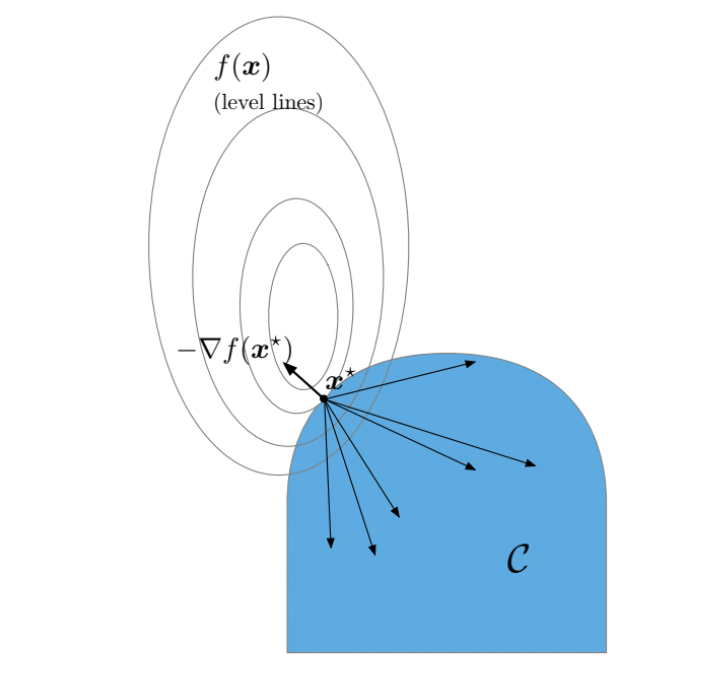
\includegraphics[width=0.6\textwidth]{figure/cp_opt_con.png}
    \caption{}
\end{figure}

\begin{proof}
    1
\end{proof}

\subsection{Examples}
The abstract geometrical result in the previous section will eventually
lead us to the Karush-Kuhn-Tucker (KKT) conditions. But we will
build up to this by looking at what it tells us in several important
(and prevalent) cases.
We assume throughout this section that $f$ is convex, differentiable,
and defined on all of $\R^n$.
\par
\noindent\bf{Linear constraints}

\noindent\bf{Non-negativity constraints}

\noindent\bf{A single convex inequality constraint}



\section{Reference}



\begin{itemize}
    \item \href{https://sites.gatech.edu/ece-6270-fall-2022/}{Constrained Minimization}
\end{itemize}
\chapter{Normal and Tangent Cones}


\section{Reference}
\begin{itemize}
    \item \href{}{CS/ISyE/Math 730: Nonlinear Optimization 2 Lecture Notes}
\end{itemize}





% \part{}


%%%%%%%%%%%%%%%Content%%%%%%%%%%%%%%%
% % \mainmatter % separat the number of toc and mainmatter
% \chapter*{Preface}

Notes mainly refer to following materials:


\begin{itemize}
    \item[*] Machine learning
    \begin{itemize}
        \item \href{https://www.cs.cornell.edu/courses/cs4780/2023sp/}{lecture notes from cornell}
        \item \href{https://www.cs.cmu.edu/~hn1/documents/machine-learning/notes.pdf}{lecture notes from cmu}
        \item \href{https://cs229.stanford.edu/main_notes.pdf}{lecture notes of CS229}
    \end{itemize}
    \item[*] Deep learning
    \begin{itemize}
        \item \href{https://udlbook.github.io/udlbook/}{understanding deep learning}
        \item \href{https://www.bilibili.com/video/BV1Wv411h7kN/?spm_id_from=333.337.search-card.all.click}{lecture video from Hongyi Lee}
        \item \href{https://cs231n.github.io/}{lecture notes from Stanford}
    \end{itemize}
    \item[*] Reinforcement learning
    \begin{itemize}
        \item \href{https://web.stanford.edu/class/cs234/modules.html}{lecture notes from stanford}
        \item \href{https://people.cs.umass.edu/~bsilva/courses/CMPSCI_687/Fall2022/Lecture_Notes_v1.0_687_F22.pdf}{lecture notes from umass}
    \end{itemize}
\end{itemize}







% \part{Mathematics}

% % !TEX root = ../notes_template.tex
\chapter{Discrete Math}\label{chp:discrete_math}


\section{Proof}

\begin{theorem}
\end{theorem}

\begin{solution}
By induction:
\end{solution}



\section{Quantifier}
\lipsum % dummy text - remove from real document

\section{Graph}
\citetitle{babaiGraphIsomorphismQuasipolynomial2016}
\cite{babaiGraphIsomorphismQuasipolynomial2016}

\section{Number theory}
Figure example
\begin{figure}[!ht]
    \centering
    \includegraphics[width=1\linewidth]{./figure/elliptic_curves.pdf}
    \caption{Elliptic curves \cite{childsUniversalComputationQuantum2009} }
\end{figure}


\section{Algorithm}
% \begin{center}
% \begin{minipage}{.9\linewidth}
% algorithm2e
% https://www.overleaf.com/learn/latex/Algorithms#The_algorithm2e_package
\begin{algorithm}[H]
    \SetKwInOut{Input}{input}
    \SetKwInOut{Output}{output}
    \Input{Integer $N$ and parameter $1^t$}
    \Output{A decision as to whether $N$ is prime or composite}
    \BlankLine
    \For{ $i = 1,2, \ldots, t$} {
        $a\leftarrow \qty{1,\dots,N_1}$\;
        \If{$a^{N-1} \neq 1 \mod{N}$}
    {\Return "composite"}
    }
    \Return "prime"
    \caption{Primality testing - first attempt}
    \label{alg:miller_rabin}
\end{algorithm}
% \end{minipage}
% \end{center}

% \part{Computer Science}
% % \input{./chapter/complexity.tex}
% % !TEX root = ../notes_template.tex
\chapter{Machine Learning}\label{chp:machine_learning}
\minitoc

\section{Regression}
% \gls{algorithm};
\subsection{Gradient descent}\label{sec:gradient_descent}
\gls{gd};
% \glsxtrshort{gd}

\section{Support Vector Machine}
\gls{svm};
% % \input{./chapter/algorithms.tex}

% \part{Physics}
% % !TEX root = ../notes_template.tex
\chapter{Quantum Mechanics}\label{chp:quantum_mechanics}
\minitoc

\section{Hamiltonian}
\gls{hamiltonian};
% \glsxtrshort{qm};

\section{Path Integral}
\gls{lagrangian}

\section{Quantum Field Theory}
\gls{qft};
% % \input{./chapter/quantum_field_theory.tex}

% % \begin{appendices}
% % % !TEX root = ../notes_template.tex
\chapter{Formulas}

\section{Gaussian distribution}\label{sec:gaussian_distribution}
\begin{Definition}[Gaussian distribution]\label{def:gaussian_distribution}
    \myindex{Gaussian distribution}
\end{Definition}

\begin{theorem}[Central limit theorem]\label{thm:central_limit_theorem}
\end{theorem}
% % \end{appendices}

% \backmatter

% %%%%%%%%%%%%%%% Reference %%%%%%%%%%%%%%%

% \printbibliography[heading=bibintoc]
% \printindex
\end{spacing}
\end{document}